\begin{figure}[!htbp]
  \centering
  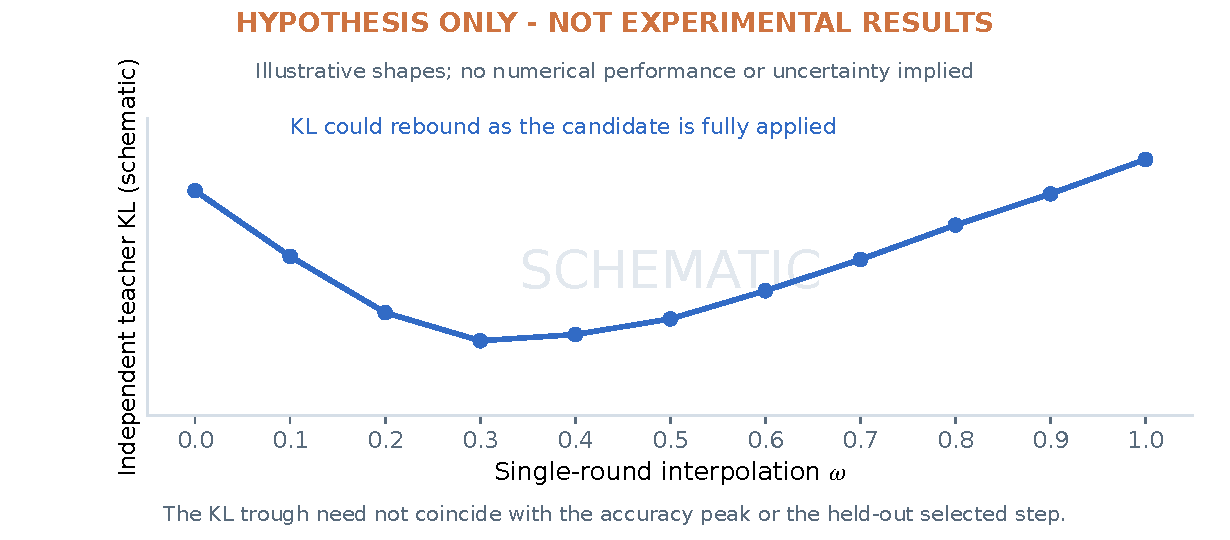
\includegraphics[width=0.78\linewidth]{figures/hypothesis_step_kl.pdf}
  \caption{\textbf{单轮步长--教师 KL 的预期趋势示意，非实验结果。}可能的情形是 KL 随小步更新降低、随后回升；不保证回升一定出现，也不保证最低点与图~\ref{fig:ink-step-size-analysis} 的准确率峰值重合。纵轴无实测 KL 数值，原留出集选步需待运行后另行标注。}
  \label{fig:ink-step-kl-analysis}
\end{figure}
